% !TEX program = lualatex
%!TEX TS-program = lualatex
\documentclass[12pt,a4paper]{article}
\usepackage{fontspec}
\usepackage{polyglossia}
\setdefaultlanguage{polish}
\usepackage{geometry}
\geometry{margin=2.1cm}
\usepackage[table]{xcolor}
\usepackage{longtable}
\usepackage{array}
\usepackage{booktabs}
\usepackage{enumitem}
\usepackage{ragged2e}
\usepackage{graphicx}
\usepackage{float}
\definecolor{tableHeader}{HTML}{E8EEF7}
\definecolor{tableStripe}{HTML}{F7F9FC}
\newcolumntype{L}[1]{>{\RaggedRight\arraybackslash}p{#1}}
\newcolumntype{C}[1]{>{\Centering\arraybackslash}p{#1}}
\renewcommand{\arraystretch}{1.22}
\setlength{\tabcolsep}{4pt}
\setlist[itemize]{leftmargin=*, itemsep=2pt, topsep=2pt}
\setlength{\parindent}{0pt}
\setlength{\parskip}{6pt}
\emergencystretch=3em
\sloppy
\begin{document}

\section*{Raport ze sprintu nr 6 - Calisia Banking App}
Data raportu: 31.05.2026

Okres sprintu: 26.05 - 31.05.2026

Product Owner / Scrum Master: Dawid Olszewski

\subsection*{Lista osób}
\begin{itemize}
\item Kubryn Jeremiasz
\item Łaszuk Jakub
\item Makarevich Ksenia
\item Nuckowski Michał
\item Ruczyńska Nikola
\item Wołczko Jakub
\item Olszewski Dawid
\end{itemize}

\subsection*{Product Owner i Scrum Master sprintu}
Dawid Olszewski

\subsection*{Sprint Planning}
\begingroup
\footnotesize
\rowcolors{2}{tableStripe}{white}
\begin{longtable}{@{}C{0.08\textwidth}L{0.62\textwidth}C{0.10\textwidth}L{0.12\textwidth}@{}}
\toprule
\rowcolor{tableHeader}
\textbf{Kod} & \textbf{Historyjka} & \textbf{SP} & \textbf{Status} \\
\midrule
\endfirsthead
\toprule
\rowcolor{tableHeader}
\textbf{Kod} & \textbf{Historyjka} & \textbf{SP} & \textbf{Status} \\
\midrule
\endhead
S6-01 & Przelew własny między rachunkami klienta & 13 & Done \\
S6-02 & Przelew zewnętrzny & 13 & Done \\
S6-03 & Panel przelewów i szybka aktualizacja dashboardu & 8 & Done \\
S6-04 & Walidacje i scenariusze negatywne przelewów & 8 & Done \\
\bottomrule
\end{longtable}
\endgroup

\subsection*{Sprint Review}
Cel sprintu: Przelewy własne i zewnętrzne. Pozwolenie klientowi na wykonywanie przelewów oraz odzwierciedlanie ich w saldach i historii.

Zakres sprintu obejmował 4 historyjek o łącznej estymacji 42 SP. Wszystkie historyjki zostały dowiezione ze statusem Done, dlatego osiągnięta prędkość sprintu wyniosła 42 SP.

Dostarczono obsługę przelewów własnych i zewnętrznych, w tym walidacje danych, obciążenie rachunku źródłowego, zapis transferu oraz aktualizację dashboardu po operacji.

Sprint domknął najważniejszą funkcjonalność operacyjną bankowości. Klient może wykonać przelew, a system utrzymuje spójność sald, historii i widoku dashboardu.

\subsubsection*{Najważniejsze rezultaty / Przyrost}
\begin{itemize}
\item Dodano przelew własny między rachunkami klienta.
\item Dodano przelew zewnętrzny na rachunek odbiorcy.
\item Połączono panel przelewów z aktualizacją dashboardu.
\item Przetestowano scenariusze negatywne i walidacje przelewów.
\end{itemize}

\subsection*{Sprint Retrospective}
Sprint 6 przypadł na okres kończącego się semestru, co dla większości członków zespołu oznaczało równoczesną realizację innych projektów, przygotowania do zaliczeń oraz zwiększoną liczbę obowiązków akademickich. Był to test naszej organizacji pracy, odpowiedzialności oraz umiejętności współpracy pod presją czasu.

Pomimo ograniczonej dostępności części zespołu udało się utrzymać dobrą komunikację i konsekwentnie realizować zaplanowane zadania. Nie prowadziliśmy formalnych spotkań Daily Scrum, jednak pozostawaliśmy w stałym kontakcie za pośrednictwem Discorda, a w razie potrzeby organizowaliśmy krótkie spotkania na Teamsie. Dzięki temu udało się ukończyć wszystkie historyjki zaplanowane na sprint i osiągnąć założony cel.

\subsubsection*{Co się udało}
\begin{itemize}
\item Wszystkie zadania zaplanowane na sprint zostały ukończone zgodnie z planem.
\item Udało się utrzymać dobrą komunikację pomimo dużej liczby obowiązków poza projektem.
\item Członkowie zespołu aktywnie wspierali się nawzajem przy rozwiązywaniu problemów.
\item Wspólne podejmowanie decyzji pozwoliło uniknąć opóźnień i sprawnie realizować zadania.
\end{itemize}
\subsubsection*{Poziom energii zespołu}
Średni poziom energii zespołu: 4,0/5.

Pomimo intensywnego okresu akademickiego poziom motywacji pozostawał wysoki. Widoczne było zmęczenie wynikające z licznych projektów i zaliczeń, jednak świadomość zbliżającego się zakończenia projektu oraz zaangażowanie wszystkich członków zespołu pozwoliły utrzymać dobre tempo pracy przez cały sprint.

\subsubsection*{Czego udało się nauczyć}
\begin{itemize}
\item Regularna komunikacja jest kluczowa nawet wtedy, gdy nie odbywają się formalne spotkania Daily Scrum.
\item Krótkie spotkania organizowane w razie potrzeby pozwalają szybciej rozwiązywać problemy niż długie dyskusje tekstowe.
\item Wzajemne wsparcie członków zespołu znacząco wpływa na terminową realizację zadań.
\item W okresach zwiększonego obciążenia obowiązkami szczególnie ważne jest realistyczne planowanie pracy i bieżące informowanie zespołu o swojej dostępności.
\end{itemize}
\subsubsection*{Wnioski i działania na kolejny sprint}
\begin{itemize}
\item Utrzymać dotychczasowy poziom komunikacji i współpracy w zespole.
\item W dalszym ciągu organizować krótkie spotkania synchronizacyjne w przypadku pojawienia się problemów.
\item Skupić się na końcowych testach całego systemu oraz eliminacji wykrytych błędów.
\item Zweryfikować spójność działania wszystkich funkcjonalności przed oddaniem projektu.
\item Przygotować aplikację oraz dokumentację do prezentacji końcowej.
\end{itemize}

\subsection*{Następny sprint}
Product Owner / Scrum Master w następnym sprincie: Nikola Ruczyńska

Główny cel następnego sprintu: Stabilizacja, testy i oddanie produktu. Dopracowanie całego przepływu klienta, usunięcie niespójności i przygotowanie produktu do prezentacji.

\subsection*{Zrzuty ekranu}

\begin{figure}[H]
    \centering
    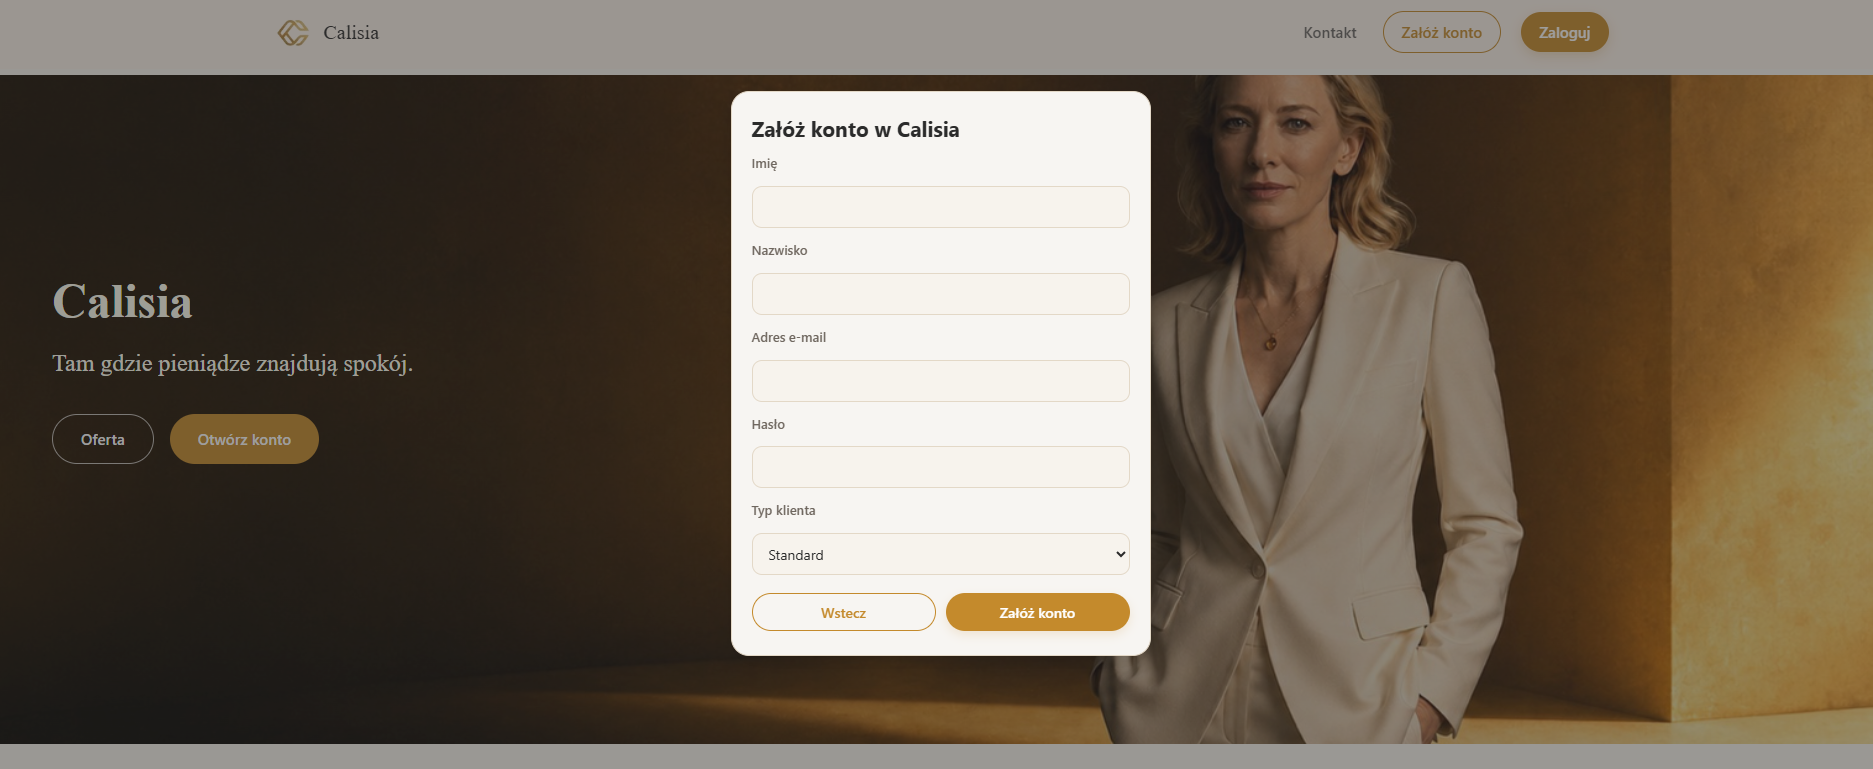
\includegraphics[width=0.95\textwidth]{assets/01_rejestracja.png}
    \caption{Rejestracja użytkownika.}
\end{figure}

\begin{figure}[H]
    \centering
    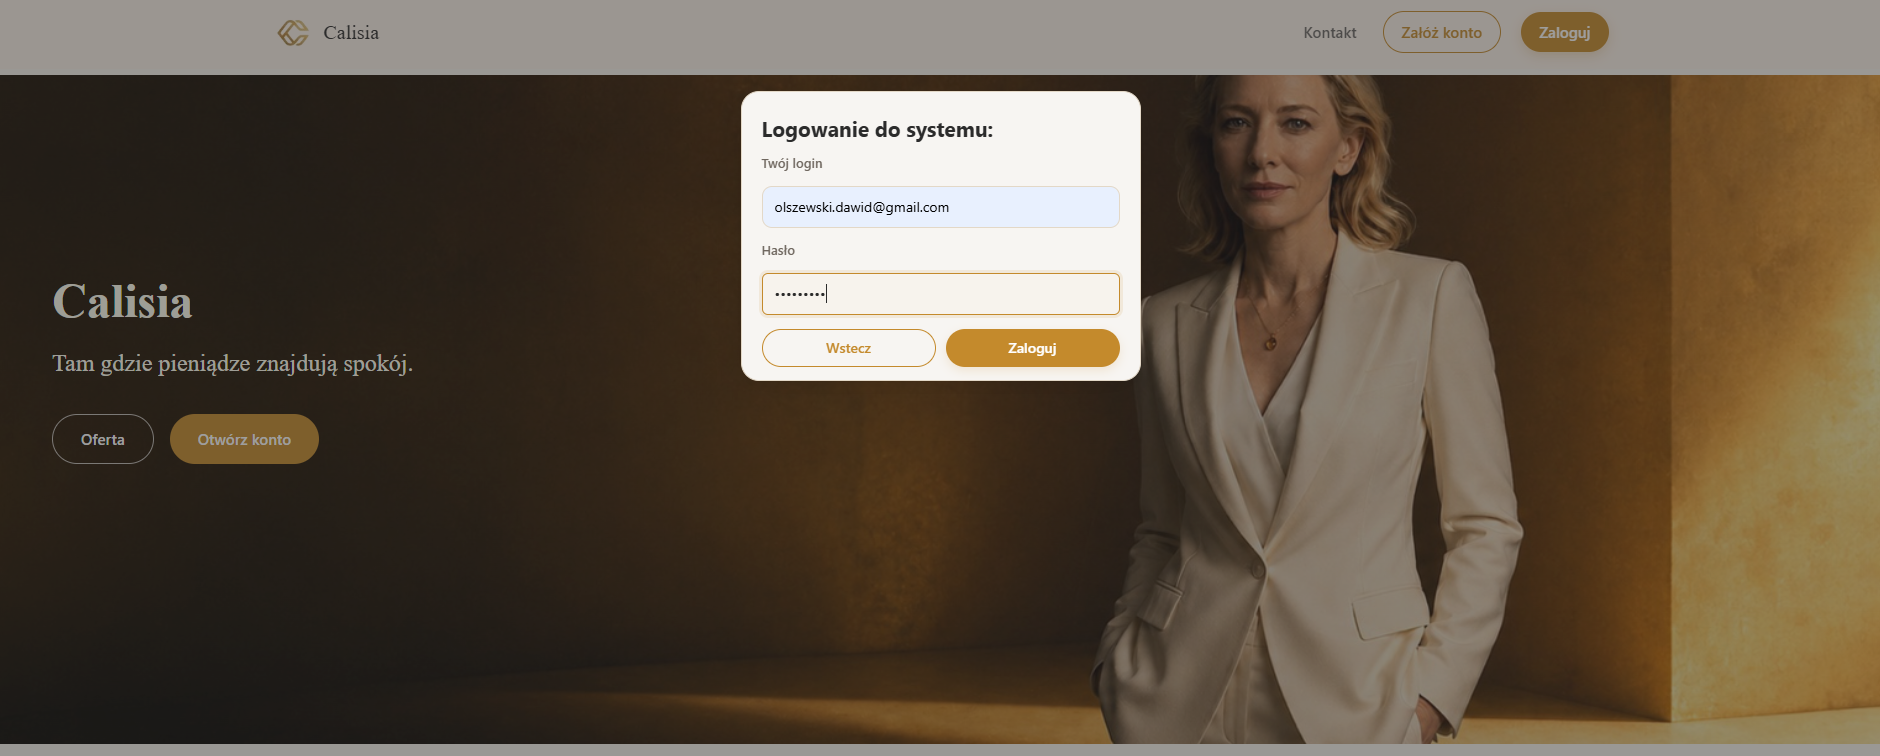
\includegraphics[width=0.95\textwidth]{assets/02_logowanie.png}
    \caption{Logowanie użytkownika.}
\end{figure}

\begin{figure}[H]
    \centering
    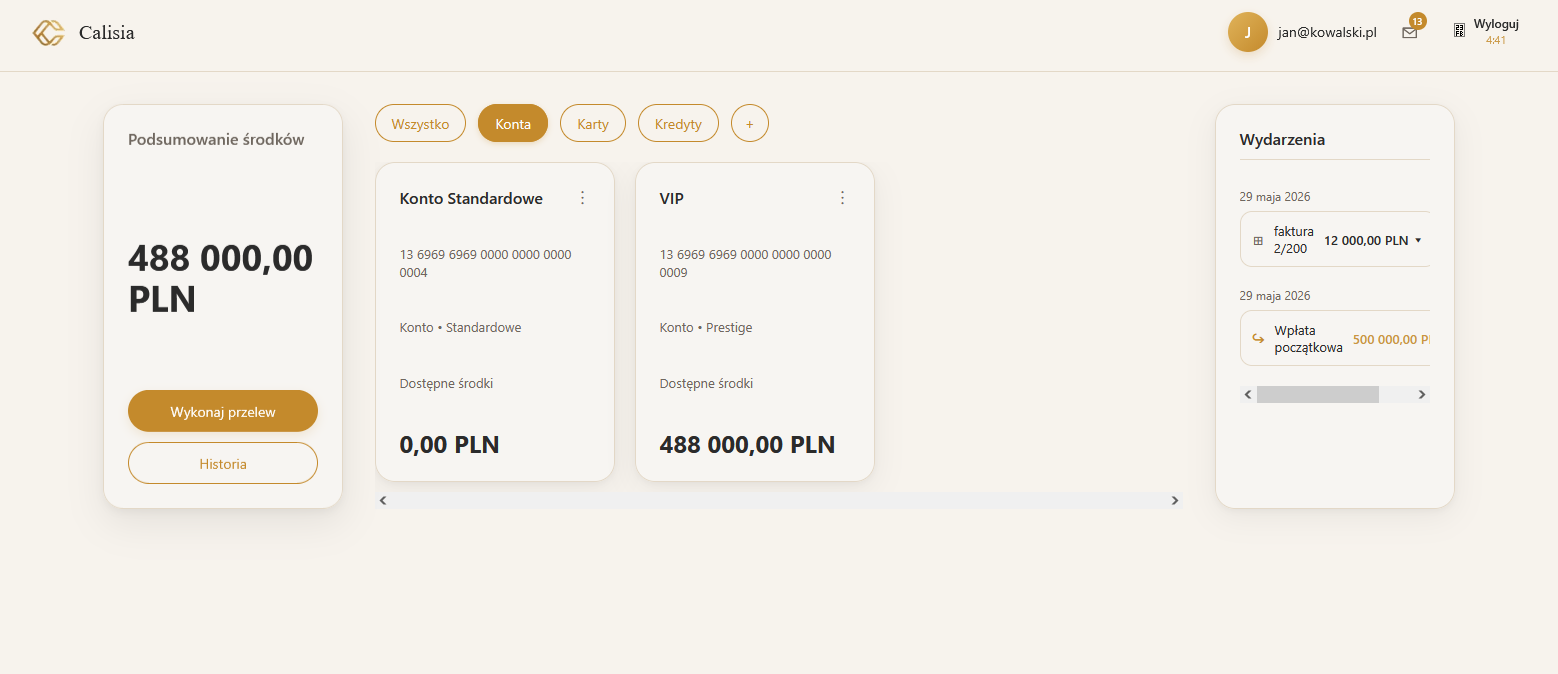
\includegraphics[width=0.95\textwidth]{assets/03_dash.png}
    \caption{Dashboard użytkownika.}
\end{figure}

\begin{figure}[H]
    \centering
    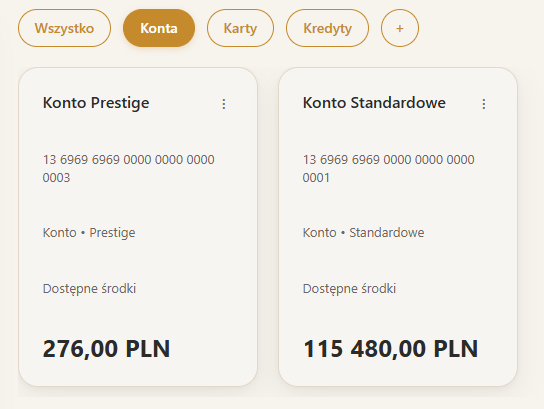
\includegraphics[width=0.95\textwidth]{assets/04_konta.png}
    \caption{Konta użytkownika.}
\end{figure}

\begin{figure}[H]
    \centering
    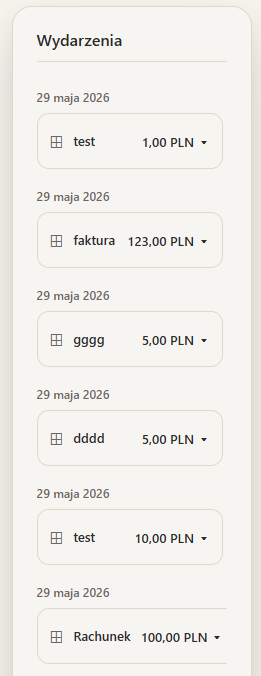
\includegraphics[width=0.5\textwidth]{assets/05_historia.png}
    \caption{Historia przelewów.}
\end{figure}

\begin{figure}[H]
    \centering
    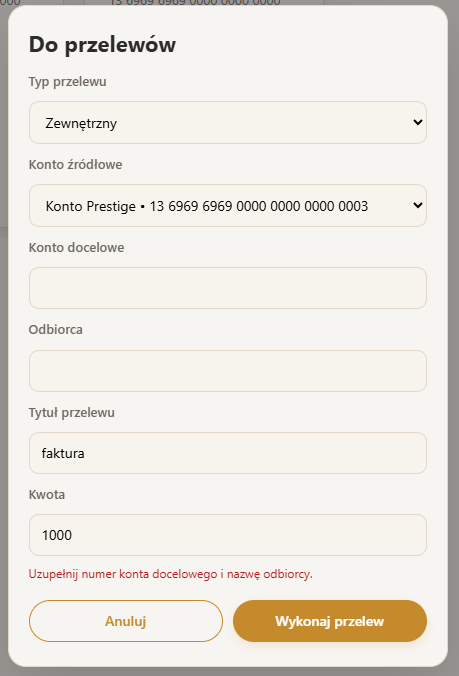
\includegraphics[width=0.95\textwidth]{assets/06_walidacja_numer_konta.png}
    \caption{Walidacja numeru konta.}
\end{figure}

\begin{figure}[H]
    \centering
    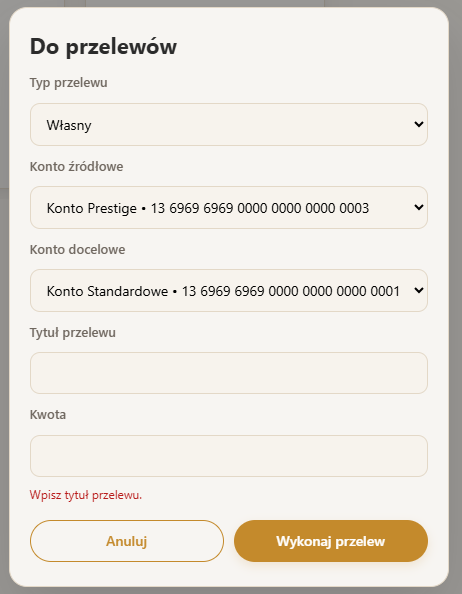
\includegraphics[width=0.95\textwidth]{assets/07_walidacja_wpisz_tytul_przelewu.png}
    \caption{Walidacja tytułu przelewu.}
\end{figure}

\begin{figure}[H]
    \centering
    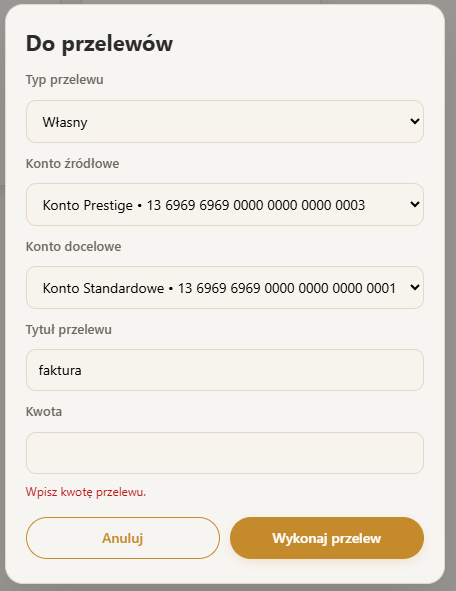
\includegraphics[width=0.95\textwidth]{assets/08_walidacja_wpisz_kwote_przelewu.png}
    \caption{Walidacja kwoty przelewu.}
\end{figure}

\begin{figure}[H]
    \centering
    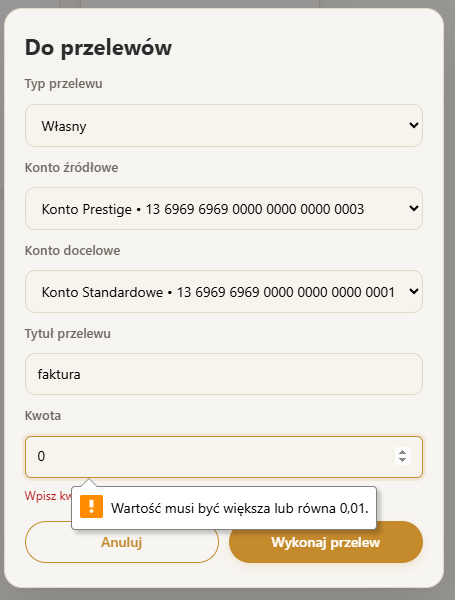
\includegraphics[width=0.95\textwidth]{assets/09_walidacja_wartosc_wiekszanizzero.png}
    \caption{Sprawdzenie, czy wartość jest większa niż zero.}
\end{figure}

\begin{figure}[H]
    \centering
    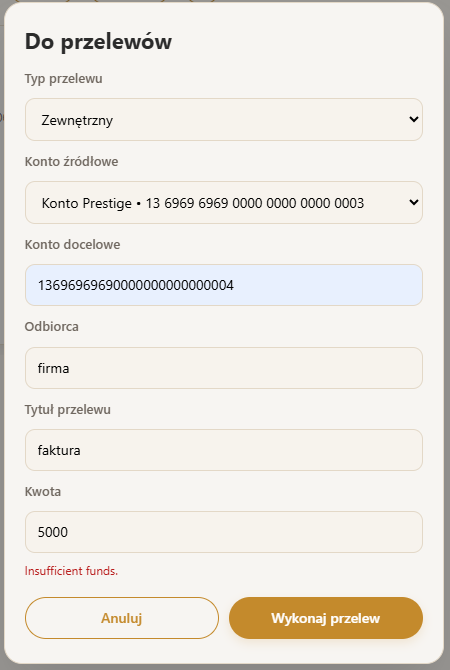
\includegraphics[width=0.95\textwidth]{assets/10_walidacja_brak_srodkow.png}
    \caption{Walidacja, czy użytkownik ma wystarczające środki.}
\end{figure}

\end{document}
